\section{Results}
\label{sec:results}

\Cref{fig:mvp} is the headline. The left panel reports the policy mean
estimand, the right panel reports $\CVaR_{0.10}$. Pale triangles are
the cheap-only baseline (no calibration). Black diamonds are the
oracle truth on the full $n_0 = 500$ panel. Colored circles are Direct
CVaR-CJE. Whiskers around each Direct estimate are 95\% percentile
confidence intervals from the full-pipeline bootstrap (resample train,
evaluation, and audit slices; refit the calibrator; re-optimize $\that$
inside every replicate; \cref{app:bootstrap}). The faint shaded band
behind \textsc{base} and \textsc{clone} marks the
indistinguishable-policy region. The two share the same model and
prompt at adjacent seeds, and Direct estimates respect that equivalence
on both estimands.

\begin{figure}[h]
\centering
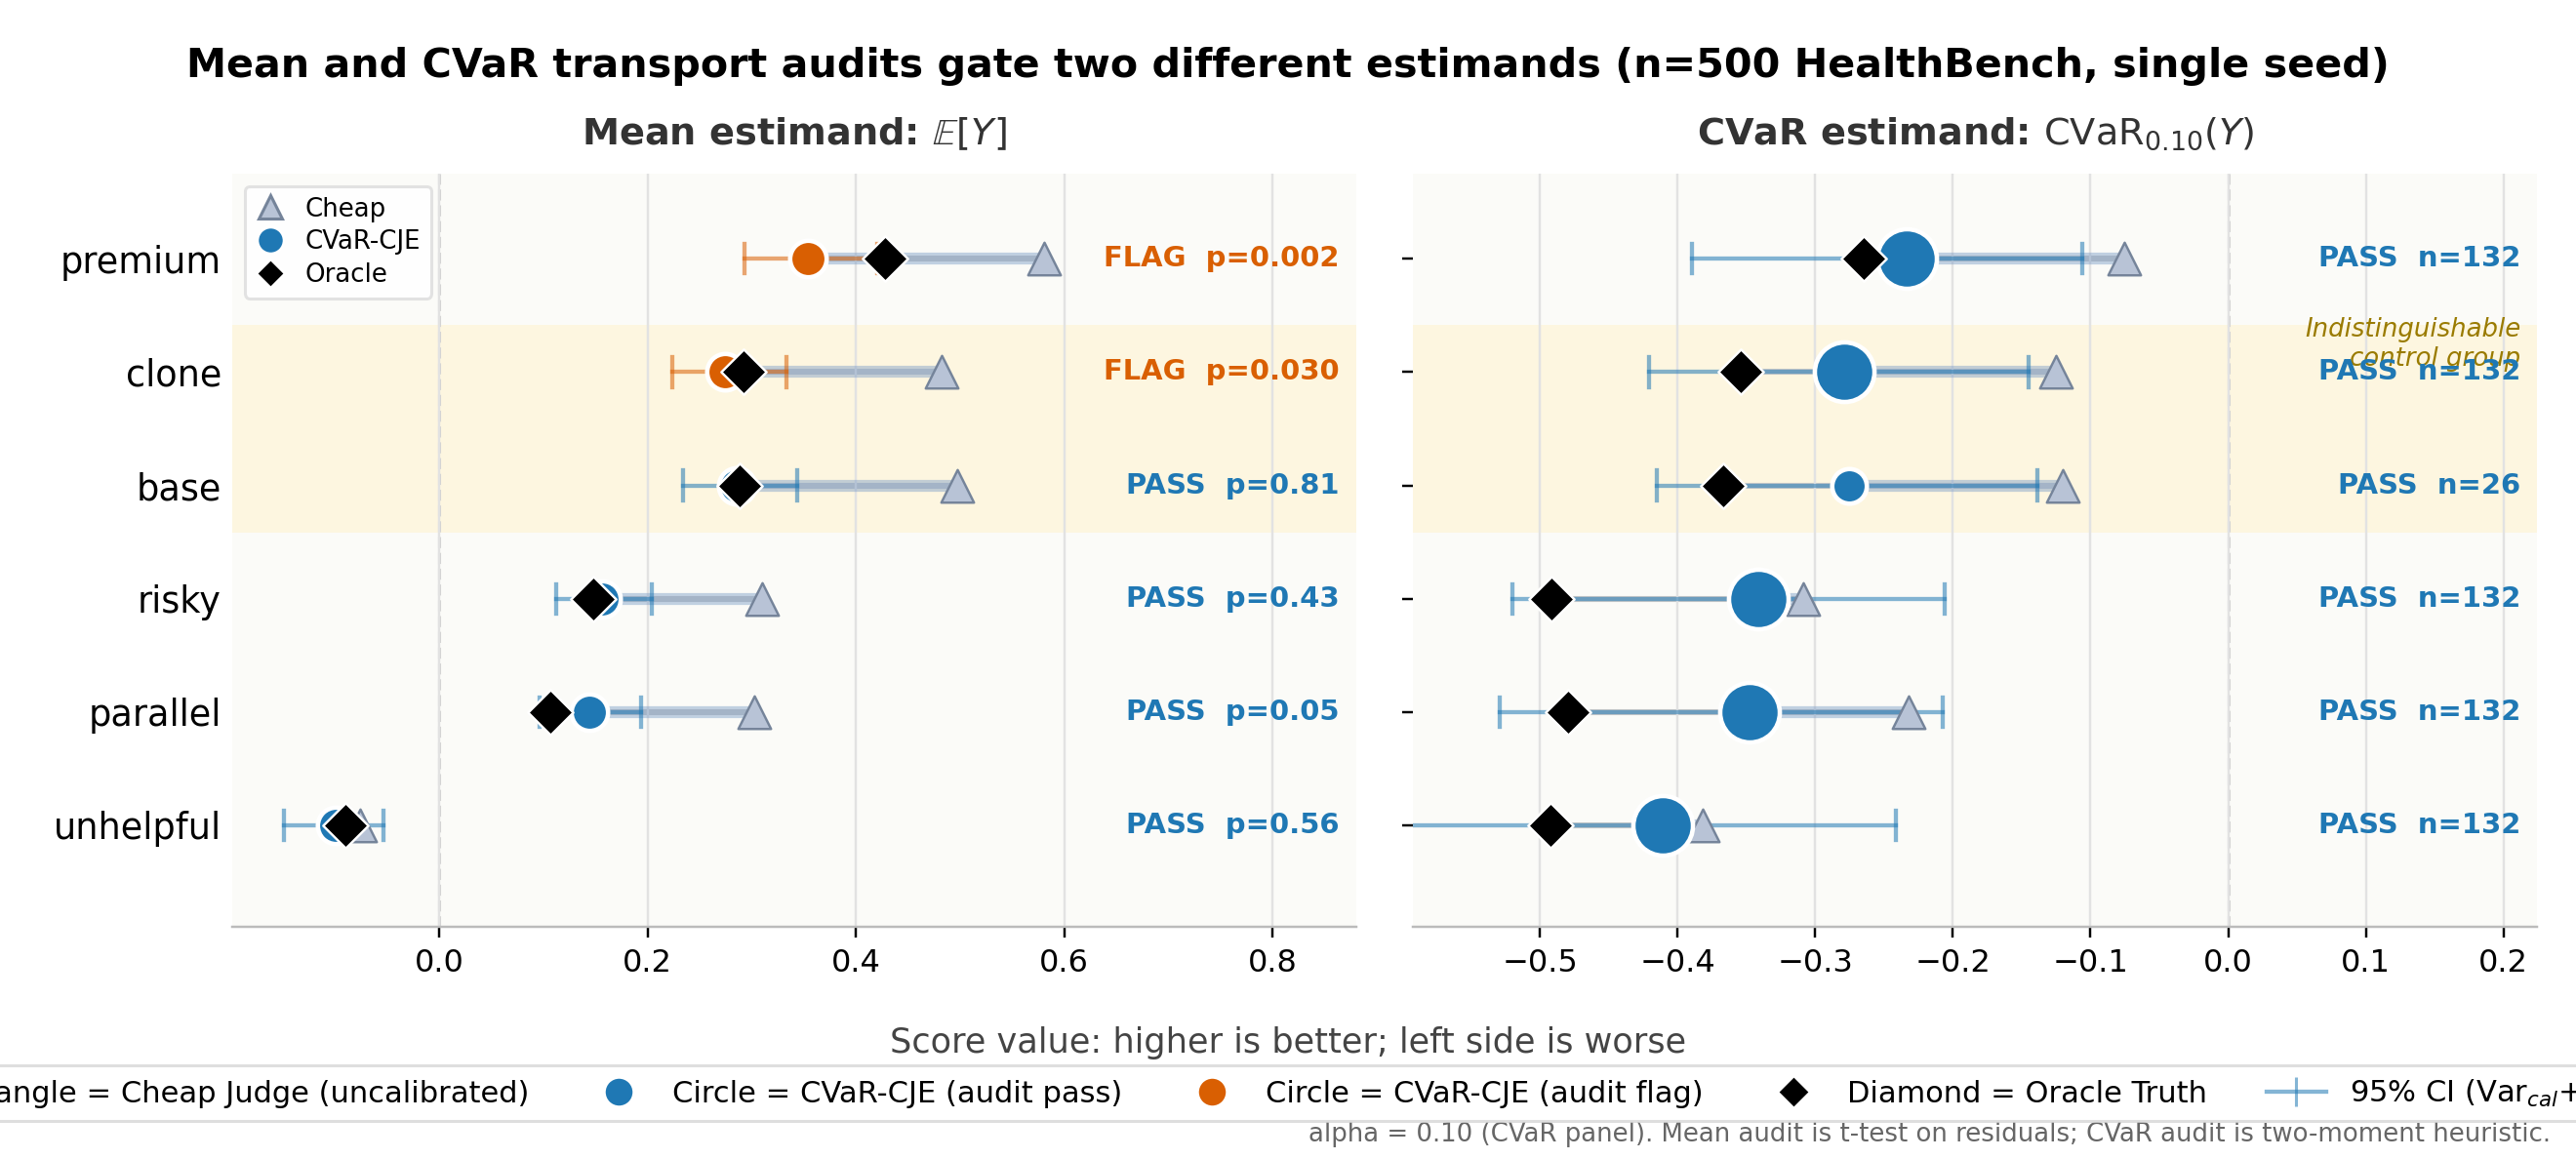
\includegraphics[width=0.95\textwidth]{healthbench_data/writeup/mvp_one_graph.pdf}
\caption{Two-panel summary on the HealthBench $n_0 = 500$ panel. Left:
mean estimand $\E_\ptarget[\Y]$, with mean-transport audit verdicts.
Right: $\CVaR_{0.10}(\ptarget)$, with the two-moment CVaR audit
verdicts. In each panel, pale triangles are the cheap-only baseline,
black diamonds are the full-oracle truth, and colored circles are the
Direct CJE estimate (blue audit pass, orange audit flag). Whiskers
around each Direct estimate are 95\% percentile confidence intervals
from the full-pipeline bootstrap that resamples train, evaluation, and
audit slices, refits the calibrator, and re-optimizes $\that$ inside
every replicate ($B = 500$; \cref{app:bootstrap}). Overlapping whiskers
between two
policies mean the policies are not statistically distinguishable at
this sample size. A pass verdict says the calibrator transports for
that policy, not that the ranking against neighbors is conclusive. The
shaded yellow band marks \textsc{base} and \textsc{clone}, which share
a model and prompt at adjacent seeds and are statistically
indistinguishable. Mean and CVaR audits test different transport
conditions and can disagree. \textsc{clone} and \textsc{premium} flag
the mean audit but pass the CVaR audit at $\alpha = 0.10$. Live
numbers in \cref{tab:alpha10,tab:alpha20}.}
\label{fig:mvp}
\end{figure}

\subsection{CVaR-CJE Fixes the Cheap Judge}
\label{sec:results-cvar}

\Cref{tab:alpha10} reports $\alpha = 0.10$ results across all five
policies. The Direct estimate beats the cheap-only baseline on every
policy. Mean absolute error against the full-oracle truth drops from
$0.204$ for cheap-only to $0.082$ for Direct, a $60\%$ reduction. The
cheap judge systematically understates how bad the worst-tail
responses are. The rubric's negative-points criteria fire harder than
gpt-4o-mini's default leniency anticipates, so cheap scores in the
tail are too high. The calibrator picks this up and pulls predictions
down. All five rows pass the audit, so all five Direct estimates count
as level claims.

\begin{table}[h]
\centering\footnotesize
\caption{$\alpha = 0.10$ results. Cheap-only is $\CVaR$ on raw cheap
scores (no calibration). \textbf{Direct CVaR-CJE} is the calibrated
estimate. Oracle truth is the atom-split $\CVaR$ on the full $n_0 = 500$
oracle panel. Audit-only $\CVaR$ is the empirical $\CVaR$ on the
$n_{\mathrm{audit}}$ oracle rows alone, with a 95\% percentile bootstrap
CI shown as the half-width $\pm$. The audit verdict gates whether the
row's Direct estimate counts as a level claim.}
\label{tab:alpha10}
\resizebox{\textwidth}{!}{
\begin{tabular}{l r r r r r r r r l}
\toprule
\thead{policy} & \thead{$\overline{\Y}$} & \thead{cheap-only\\ $\CVaR$} & \thead{\textbf{Direct}\\ \textbf{CVaR-CJE}} & \thead{audit-only\\ $\CVaR$\\ ($\pm$ half-CI)} & \thead{Oracle\\ Truth} & \thead{abs.\ error\\ of Direct} & \thead{$\bar g_1$} & \thead{$\bar g_2$} & \thead{audit\\ verdict} \\
\midrule
\textsc{base}      & $+0.289$ & $-0.120$ & $\mathbf{-0.276}$ & \makecell[r]{$-0.299$\\ $\pm 0.250$} & $-0.367$ & $0.091$ & $-0.023$ & $+0.006$ & \textsc{pass} \\
\textsc{clone}     & $+0.292$ & $-0.125$ & $\mathbf{-0.279}$ & \makecell[r]{$-0.245$\\ $\pm 0.089$} & $-0.354$ & $0.075$ & $-0.002$ & $-0.005$ & \textsc{pass} \\
\textsc{premium}   & $+0.428$ & $-0.076$ & $\mathbf{-0.233}$ & \makecell[r]{$-0.223$\\ $\pm 0.120$} & $-0.264$ & $0.031$ & $+0.006$ & $-0.003$ & \textsc{pass} \\
\textsc{parallel}  & $+0.106$ & $-0.232$ & $\mathbf{-0.348}$ & \makecell[r]{$-0.475$\\ $\pm 0.152$} & $-0.479$ & $0.132$ & $+0.044$ & $+0.013$ & \textsc{pass} \\
\textsc{unhelpful} & $-0.090$ & $-0.382$ & $\mathbf{-0.411}$ & \makecell[r]{$-0.371$\\ $\pm 0.063$} & $-0.492$ & $0.081$ & $+0.044$ & $-0.003$ & \textsc{pass} \\
\midrule
\multicolumn{2}{l}{\itshape mean abs.\ error} & $0.204$ & $\mathbf{0.082}$ & & & & & & \\
\bottomrule
\end{tabular}
}
\end{table}

\paragraph{Tail and mean line up where they should.}
\textsc{base} and \textsc{clone} differ in mean oracle score by
$0.003$ and in $\CVaR_{0.10}$ truth by $0.013$. The Direct estimates
match this indistinguishability: $-0.276$ vs.\ $-0.279$ on the
calibrated $\CVaR$, inside any reasonable noise band. \textsc{premium}
sits cleanly above the \textsc{base}/\textsc{clone} cluster on both
estimands (mean $+0.428$, $\CVaR$ $-0.233$). \textsc{parallel} and
\textsc{unhelpful} sit cleanly below, with $\CVaR$ separations far
exceeding their mean separations. The gap between \textsc{premium} and
\textsc{unhelpful} is $0.518$ on the mean panel and $0.178$ on the
$\CVaR$ panel.

\paragraph{Visual proof of calibration.}
\Cref{fig:tailcdf} zooms on the bottom-$20\%$ region of the score
distribution for the two stress-test policies (\textsc{parallel} and
\textsc{unhelpful}). Each panel overlays three empirical CDFs:
cheap-$\Sscore$ (blue), oracle-$\Y$ (red), and CJE-calibrated
$\hat f(\Sscore)$ (green). The cheap CDF sits to the right of the
oracle CDF on both policies. The cheap judge is too lenient in the
tail. On \textsc{parallel} the calibrated $\hat f(\Sscore)$ curve
closely tracks the oracle CDF in the zoomed region. The isotonic
stop-loss calibrator reconstructs the true tail shape. On
\textsc{unhelpful} the calibrated curve is monotonically below the
cheap curve and roughly overlays the oracle curve. This is the
picture Table 1 summarizes in one cell.

\begin{figure}[h]
\centering
\includegraphics[width=0.95\textwidth]{healthbench_data/writeup/tail_cdf.pdf}
\caption{Bottom-$20\%$ tail CDFs for \textsc{parallel} and
\textsc{unhelpful} at $\alpha = 0.10$. Cheap-$\Sscore$ (blue) is
shifted right of oracle-$\Y$ (red). The CJE-calibrated $\hat f(\Sscore)$
curve (green) overlays the oracle curve in the tail region. Vertical
dashed lines mark $t^\star$ (atom-split oracle $\alpha$-quantile, see
\cref{app:estimands}). Dotted lines mark the corresponding cheap-baseline
quantile. Horizontal line at $F = \alpha$.}
\label{fig:tailcdf}
\end{figure}

\subsection{The Audit Catches the Adversarial Policy}
\label{sec:results-audit}

\cref{tab:alpha20} repeats the analysis at $\alpha = 0.20$. Direct
again beats cheap-only everywhere. Four of five rows pass the audit.
The exception is \textsc{unhelpful}. Its empirical tail mass at the
selected threshold is $36\%$ instead of the $20\%$ the calibrator
implies ($\bar g_1 = +0.164$, $48/132$ audit rows below $\hat t_\alpha$
vs.\ expected $26.4$, two-sided binomial $p < 10^{-3}$). The audit
refuses to call $-0.297$ a $\CVaR_{0.20}$ level for \textsc{unhelpful}.

\begin{table}[h]
\centering\footnotesize
\caption{$\alpha = 0.20$ results. Same column definitions as
\cref{tab:alpha10}. \textsc{unhelpful} flags on $\bar g_1$. Empirical
tail mass at $\hat t_\alpha$ is $36\%$ instead of the $20\%$ the
calibrator implies, two-sided binomial $p < 10^{-3}$. The cell shows
the numeric estimate but is not a level claim.}
\label{tab:alpha20}
\resizebox{\textwidth}{!}{
\begin{tabular}{l r r r r r r r r l}
\toprule
\thead{policy} & \thead{$\overline{\Y}$} & \thead{cheap-only\\ $\CVaR$} & \thead{\textbf{Direct}\\ \textbf{CVaR-CJE}} & \thead{audit-only\\ $\CVaR$\\ ($\pm$ half-CI)} & \thead{Oracle\\ Truth} & \thead{abs.\ error\\ of Direct} & \thead{$\bar g_1$} & \thead{$\bar g_2$} & \thead{audit\\ verdict} \\
\midrule
\textsc{base}      & $+0.289$ & $+0.024$ & $\mathbf{-0.149}$ & \makecell[r]{$-0.156$\\ $\pm 0.208$} & $-0.197$ & $0.049$ & $-0.008$ & $+0.008$ & \textsc{pass} \\
\textsc{clone}     & $+0.292$ & $+0.020$ & $\mathbf{-0.153}$ & \makecell[r]{$-0.141$\\ $\pm 0.069$} & $-0.185$ & $0.032$ & $+0.027$ & $-0.006$ & \textsc{pass} \\
\textsc{premium}   & $+0.428$ & $+0.084$ & $\mathbf{-0.116}$ & \makecell[r]{$-0.104$\\ $\pm 0.086$} & $-0.101$ & $0.016$ & $-0.018$ & $-0.006$ & \textsc{pass} \\
\textsc{parallel}  & $+0.106$ & $-0.119$ & $\mathbf{-0.237}$ & \makecell[r]{$-0.329$\\ $\pm 0.102$} & $-0.322$ & $0.086$ & $+0.042$ & $+0.018$ & \textsc{pass} \\
\textsc{unhelpful} & $-0.090$ & $-0.288$ & $\mathbf{-0.297}$ & \makecell[r]{$-0.305$\\ $\pm 0.044$} & $-0.363$ & $0.066$ & $\mathbf{+0.164}$ & $+0.008$ & \textbf{\textsc{refuse-level}} \\
\bottomrule
\end{tabular}
}
\end{table}

\paragraph{The refusal that mattered.}
The Direct estimate for \textsc{unhelpful} at $\alpha = 0.20$ is
$-0.297$. The truth is $-0.363$. That number would have been a
$0.066$-magnitude miss reported as a level. The audit's tail-mass
deviation flags it loudly, and the cell goes \textsc{refuse-level}.
The conclusion changes from a specific bad number to a refusal. We
cannot certify a $\CVaR$ level claim for \textsc{unhelpful} at this
tail, and we say so. This is the safety mechanism the method was
designed for.

\paragraph{Audit truth across the panel.}
We have full oracle labels on every row, so we can ask whether the
audit verdicts agree with reality. Eight of
ten cells land in the \textsc{pass}+low-error quadrant. One cell is
\textsc{pass}+high-error: \textsc{parallel} at $\alpha = 0.10$, where
the moments are inside the $0.05$ heuristic but the level error
happens to be $0.132$. One cell is \textsc{refuse-level}+low-error:
\textsc{unhelpful} at $\alpha = 0.20$, where the audit catches a
genuine transport break even though the numerical level error happens
to be only $0.066$. There are no true-catch-with-high-error cells on
this panel because the calibrator performs reasonably across all five
policies. The audit's job here is the single
\textsc{unhelpful}+$\alpha=0.20$ refusal.

\subsection{Variance Reduction and Cost-Equivalence}
\label{sec:results-cost}

A natural skeptic asks: if we already paid for the
$n_{\mathrm{audit}} = 132$ oracle labels, why not skip the cheap
judge and report the empirical $\CVaR$ on those oracle rows directly?
The audit-only column in \cref{tab:alpha10} answers this. On
\textsc{base} the audit-only $\CVaR$ has $n_{\mathrm{audit}} = 26$ and
a wild $\pm 0.250$ half-CI. Matching Direct's total variance
$\sigma^2_{\mathrm{direct}} = \Var_{\mathrm{cal}} +
\Var_{\mathrm{audit}}$ would require $N_{\mathrm{equiv}} \approx 99$
pure-oracle rows, so Direct is roughly $\mathbf{3.8\times}$ cheaper
than audit-only at this slice budget. At $\alpha = 0.20$ the same
calculation gives $\mathbf{4.6\times}$.

On \textsc{clone}, \textsc{premium}, and \textsc{parallel} at
$n_{\mathrm{audit}} = 132$, audit-only is in the same ballpark or
tighter than Direct. HealthBench's heavily-tied bottom-mass makes the
empirical $\CVaR$ on $132$ oracle rows unusually stable, and the
calibrator's resampling variance on the $80\%$ training portion
($n = 106$) dominates. On \textsc{unhelpful}, whose calibrator is the
most unstable on the panel, audit-only is markedly tighter.

The reading is straightforward. The cheap-judge calibrator buys
precision when oracle data is scarce and the calibrator is
well-conditioned. When oracle data is abundant and the calibrator is
unstable, going pure-oracle is fine. The calibrator's value in those
cases is the audit-gated level certificate itself, not the variance
reduction. That certificate is exactly what catches \textsc{unhelpful}
at $\alpha = 0.20$.

\paragraph{Compute cost.}
The full-pipeline bootstrap (calibration plus threshold scan plus
$B = 2{,}000$ replicates with $\hat t_\alpha$ re-optimized inside
each replicate) runs in under $30$ seconds per policy on a laptop on
this $n_0 = 500$ panel. That is negligible compared to the API cost
of additional oracle calls.
